\section{RC Week 6}
\subsection{Engineering correctness: Testing}
\begin{frame}{The definitive correctness myth}
We quote the following words from one of yours (@LukeXuan)
\begin{quotation}
	While testing did indeed help your code to behave correctly in most cases. It never gives full assurance. I think you should recommend the technology of formal methods, especially verification, to introduce the possibility of complete correctness of program to students.
\end{quotation}
Despite the obvious taunt in the words, these comment DOES speaks some, truth, that is:
\begin{center}
	\structure{It is fundamentally impossible, proved in theory, to guarantee the absolute \textit{correctness} of the program by simply testing it.}
\end{center}
After all testing is an attempt to engineer correctness. It is an engineer method that aims at decreasing chances of software malfunction in the field, i.e. reliability.
\end{frame}

\begin{frame}{Two general strategies in testing}
\begin{block}{Black box testing}
	Treat your program under testing as a ``blackbox". The tester cares only about input and output. Essentially our OJ does black-box testing.
\end{block}
\begin{block}{Glass box testing}
	Tester designs the test case according to the case. Test-cases are designed in such way that attempts to
	\begin{itemize}
		\item Achieve full coverage (Activate every branch once).
		\item Touch boundaries, base cases, or data-type boundaries.
		\item Stress the implementation, or exploit it for security reasons.
	\end{itemize}
\end{block}
\alert{Testing is always an active activity}, even for black box testing. Test cases are always designed with the technicals in heart.
\end{frame}


\begin{frame}{Input Partitioning}
The purpose of the testing, in most common cases, is to reveal possible defects, be trying to pick representative inputs. 

The basic logic in designing test-cases is 
\begin{center}
	\structure{If this program works on X, so it should work on Y.}
\end{center}

The job of the tester is often to categorize all possible inputs into different \textit{equivalent classes} (if you still remember that term from VE203). For each equivalent class we pick a few inputs and assume if the function works for those input, it should work for all inputs within that class.

\vspace{0.1in}
Remember, again, \alert{testing is an creative process} that relies on your understanding of both the problem and implementation at hand. 

\vspace{0.1in}
It is never an easy job to partition the input right. 
\end{frame}

\begin{frame}[fragile]{Program under testing}
The following program takes a string (of less than 100 characters) and decides whether it is palindromic recursively:
\begin{minted}{c++}
bool isPalindrome(const char* str, int size) {
    if (size == 0) return true;
    if (size == 1) return true;
    if (str[0] != str[size - 1]) return false;
    return isPalindrome(++str, size - 2);
}
int main() { 
    char str[100]; cin >> str;
    int size = strlen(str);
    cout << isPalindrome(str, size);
}
\end{minted} 
\end{frame}

\begin{frame}{Test Cases Designing: ``Normal Input"}
The most common kind of test cases are ``Normal Inputs".  Normal inputs are considered normal in the following sense:
\begin{itemize}
	\item They are normal in range. 
	\item They are normally constructed, i.e. are not delicated constructed to sabatotage / overload the program.
	\item They cover most normal outputs. 
\end{itemize}
For our previous example some good test cases will be:
\begin{itemize}
	\item \texttt{"12321"} Odd size palindrome
	\item \texttt{"1221"} Even size palindrome
	\item \texttt{"1222"} Even size non-palindrome
	\item \texttt{"1234345"} Odd size non-palindrome
\end{itemize}
\end{frame}

\begin{frame}{Test Cases Designing: ``Boundary Input"}
Boundary cases are those input that pushes the program to the ``boundary":
\begin{itemize}
	\item They are base case in recursion. 
	\item They pushes program to the edge of used datatype range.
	\item Any point that is ``tricky". For example in a \texttt{gcd} program you should remember to test the input where one argument is a multiple of another. Any input that will trigger a special treatment.
\end{itemize}
For our previous example some good test cases will be:
\begin{itemize}
	\item \texttt{""} Empty string
	\item \texttt{"1"} Single character string
	\item \texttt{123...321} 99 characters string, why 99?
	\item \texttt{"11"} Odd number (possibly) base case
\end{itemize}
\end{frame}

\begin{frame}{Test Cases Designing: ``Random / Malicious input"}
Those are inputs that does not make sense. You normally don't expect your users to supply such arguments, but often technically they can. 

For example you won't expect the user to input \texttt{I love lemonade} in a text box labeled \textit{What is your social security number?}. But technically your program can receive such input. 

It is often these situation that brings about the most trouble. These input can potentially crash the program. Or worse, construct special input that corrupts / extracts confidential data.

The conclusion is: \alert{Never trust your user, not a single byte!}
\begin{itemize}
	\item Random input, random bytes...
	\item Malicious input. 
	\item Assume that your user will not listen to your warnings. E.g. input more than 10 characters when prompted \texttt{Input a string of less than 10 characters :}.
\end{itemize}
\end{frame}

\begin{frame}{Test Cases Designing: Design with abstraction}
It is very important to keep the abstraction, or specification in general in mind when trying to design test cases.
\begin{itemize}
	\item The specification specifies the what inputs are ``normal", i.e. what are the inputs that fits ``REQUIRES" clause.
	\item The specification specifies the expected output. 
	\item The specification often defines boundaries, the one value that divides valid input with invalid inputs.
	\item The specification often suggests program load in real world.
	\item The specification tells what inputs are considered ``invalid". 
\end{itemize}
There is one more thing, the ``MODIFIES" clause. Often the code under testing produce (or relies on) side-effects. The ``MODIFIES" clause specify these things.

\alert{Again we emphasize the importance of creating a clear abstraction!}
\end{frame}

\begin{frame}{A QA (Quality Assessment) engineer walks into a bar}
The following is adapted from the work of \textit{Bill Sempf}'s twitter.
\vspace{0.1in}
A QA engineer walks into a bar
\begin{itemize}
	\item Then he orders 0 beers.
	\item Then he orders 2 beers.
	\item Then he orders 999999999999 beers.
	\item Then he orders an \texttt{aardvark}.
	\item Then he orders \texttt{nullptr}.
	\item Then he orders -1 beers.
	\item Then he orders \texttt{3.14} beers.
	\item Then he orders \texttt{asnwikfjsdf}.
	\item Then he orders \texttt{><script>giveMeCreditCard()</script>}.
	\item Finally, the QA engineer leaves without paying, comes back, and asks for the tab.
\end{itemize}
\end{frame}

\begin{frame}{\textit{Unit test}, \textit{Regression test} and \textit{Integration Test} }
\framesubtitle{Rome is not built over night. So are softwares.}

We now introduce you to some software engineering terms.

\begin{itemize}
	\item Often software are first designed by an architect, partitioned into \textit{modules}s.
	\item Programmers code each module independently. They write \texttt{Unit Tests} for each module.
	\item When the modules are put together, architect team creates \textit{Integration tests}
	\item The collection of test cases are called a \textit{Test Suite}
	\item The team will keep updating the software. After each change, a test suite a will be run to ensure the change didn't happen to break anything. This is called a \textit{Regression Test}
\end{itemize}
\end{frame}

\begin{frame}{Test automation}
From you own experience:
\begin{itemize}
	\item Testing is actually pretty common task.
	\item It takes time to create driver programs to run the tests.
	\item It takes time (and code) to create test cases. You often need to manually calculate the expected output.
	\item It takes time (and code) to analyze test results. To keep track what goes wrong, especially you.
\end{itemize}
This calls for \textit{Test Automation} and \textit{Testing Framework}s, a testing framework is (often) a piece of library that does the following:
\begin{itemize}
	\item Runs test cases automatically.
	\item Manages the test cases, selects what to run and what not.
	\item Automatically sets-up the test environment (test fixtures).
	\item Automatically keeps track of what's OK and what goes wrong.
	\item And much more...
\end{itemize}
\end{frame}

\begin{frame}[fragile]{\textit{Google Test} framework}
Project Homepage: \texttt{https://github.com/google/googletest}
Introduction is available if you  \hyperlink{https://github.com/google/googletest/blob/master/googletest/docs/Primer.md}{click here}

Here is a portion of code I used to test my VE281 project:
\begin{minted}{c++}
TEST_P(SelectionTest, DSelection) {
    int *d= dataset->getCopied();
    int size = dataset->getSize();
    for (int i = 0; i < size; ++i) {
        int val = deterministicSelection(d, size, i);
        int answer = dataset->select(i);
        ASSERT_EQ(val, answer);
        delete[] d;
        d = dataset->getCopied();
    }
    delete[] d;
}
\end{minted}
\end{frame}

\begin{frame}[fragile]{\textit{Google Test} framework}
Project Homepage: \texttt{https://github.com/google/googletest}
Introduction is available if you  \hyperlink{https://github.com/google/googletest/blob/master/googletest/docs/Primer.md}{click here}

Here is a portion of code I used to test my VE281 project:
\begin{minted}{c++}
TEST_P(SelectionTest, DSelection) {
int *d= dataset->getCopied();
int size = dataset->getSize();
for (int i = 0; i < size; ++i) {
int val = deterministicSelection(d, size, i);
int answer = dataset->select(i);
ASSERT_EQ(val, answer);
delete[] d;
d = dataset->getCopied();
}
delete[] d;
}
\end{minted}
\end{frame}

\begin{frame}{Google Test in CLion}
\vspace{-0.2in}

\begin{figure}
	\centering
	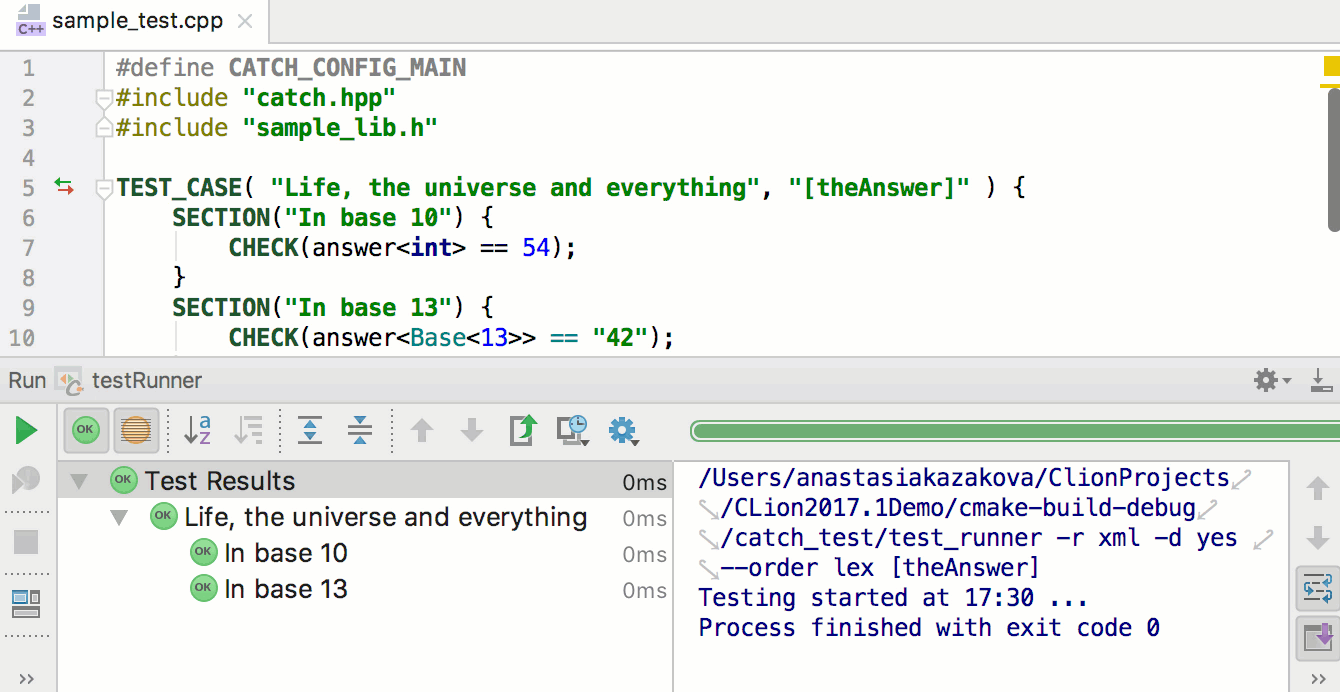
\includegraphics[scale=0.25]{fig/rc6gtest}
\end{figure}
\end{frame}

\subsection{Engineering robustness: Exceptions}
\begin{frame}{Breaking the abstraction}
The central question that goes around with exceptions are:
\begin{center}
	\structure{What if assumptions of an abstraction is broken?}
\end{center}
Note that this should be understand in a broader sense. Any program runs under some assumption. For example, 
\begin{itemize}
	\item There is enough system memory for your program.
	\item There is enough space when you need to create a file.
	\item Input outside \texttt{REQUIRES} clause never happens. 
	\item Your computer have an available Internet connections.
	\item ...
\end{itemize}
All these things constitutes the assumption you made about your abstractions. But it certainly could happen that one (or more) of them are broken. This could due to hardware limitations, or more likely due to an error in programming. 
\end{frame}

\begin{frame}[fragile]{Fail-fast \& ``I give up."}
\alert{There is absolutely no point to save a flawed processess}. This is called the fail-fast fast.
\begin{itemize}
	\item The program is already in an non-recoverable state
	\item It is probably due to a programming error
	\item Error might propagate, crash site far from source.
	\item May corrupt data. Programs can be fixed, data can't.
	\item Best strategy is to quit gracefully.
\end{itemize}
A typical situation:
\begin{minted}{c++}
void foo() {
	int *p = malloc(sizeof(int) * 10);
	// This should always success unless lacking memory
	assert(!p);
	// Do something with p
	free(p);
}
\end{minted}
\end{frame}

\begin{frame}[fragile]{``It's my problem."}
The attempt is to make the function essentially a ``total" function. Essentially this strategy says 
\begin{center}
	\structure{``Invalid inputs are part of my abstraction"}
\end{center}
Which also implies testing for invalid inputs! An (not so good) example:
\begin{minted}{c++}
// Checks if all letters ina string are capital
bool isAllCapital(char* str, int size) {
    int len = strlen(str);
    if (size != len + 1) len = size; // Input validation
    for (int i = 0; i <= len; i++) 
        if (*str < 'A' || *str > 'Z')
            return false;
    return true;
}
\end{minted}
\end{frame}

\begin{frame}{``It's my problem."}
There are some serious problem with this approach:
\begin{itemize}
	\item Function might not have well defined ``default" value. 
	\item It might hard to guess a ``default" value. 
\end{itemize}
Regardless above problem, much more serious problem comes with error propagation. There is probably a reason why this input is valid. It's most likely because you code is incorrect (in some sense) or your running environment is problematic (stack overflowed, for example).

You need to understand whenever you took this approach, you are trying to fix an already ``broken" program, going against the fail-fast principal.

\begin{itemize}
	\item You could end up crashing somewhere far from the root cause.
	\item Your program could behave wired. Since your abstraction includes treatment of ``special cases"
\end{itemize}
\end{frame}

\begin{frame}[fragile]{``It's not my problem"}
The problem of above approaches is significant because they are trying to deal with errors that does not come from themselves. The root cause of these invalid inputs are somewhere else, probably only known by their caller. 

The natural idea would be to find a method to pass the information up the chain of calling, a natural way of doing so is by return \textit{Error Codes}.

There are in general two ways to do so:
\begin{minted}{c}
// Returns negative value if error
int fact1(int n);
// Returns value signifies error, zero indicates no error
// Actual result is put into *rst 
int fact2(int n, int* rst);
\end{minted}
In some cases libraries use a global variable to store the error code of last function call.
\end{frame}

\begin{frame}[fragile]{Problem with error codes}
Both methods have severe draw back:
\begin{minted}{c++}
double tan(double rad);
\end{minted}
Function \texttt{fun} could return anything in \texttt{double}, now what should you use for error code?
\begin{minted}{c++}
int foo(double rad) {
    double rst = 0.0;int err = tan(rad, &rst);
}
\end{minted}
The second makes calling ``unnatural. Also performance drawbacks. 
\begin{itemize}
	\item Error code can be ignored. The worse thing than crashing on errors is an unattended error
	\item Error code needs to be passed up the stream. Sometimes the direct caller also don't have a clue, it needs to pass it on. 
	\item Breaks abstraction.
\end{itemize}
\end{frame}

\begin{frame}[fragile]{Structural Error handling: \texttt{try}, \texttt{catch} and \texttt{throw}}
We know introduce you to \textit{Structural Error Handling}. 
\begin{minted}{c++}
try {
    cout << "hello!" << endl; throw 123;
    cout << "Goodbye" << endl;
} catch (int x) {
   cout << "Integer Exception";
}
\end{minted}
Prints \texttt{"Hello//Interger Exception"}
\begin{itemize}
	\item A \texttt{throw} clause raise an exception (of arbitrary type).
	\item When an exception is raise, immediate stop the following execution and go for smallest enclosing \texttt{try} block.
	\item If there isn't one, terminates program.
	\item If there is one, begin matching \texttt{catch} clauses.
	\item If found, we say the error is \textit{handled}, begin executing after \texttt{try}. If not, terminates program.
\end{itemize}
\end{frame}

\begin{frame}[fragile]{Structural Error handling: \texttt{try}, \texttt{catch} and \texttt{throw}}
A try block can be matched no matter how deep in the function. The following example is just for demonstration! \alert{It is NOT a good practice!}
\begin{minted}{c++}
int foo(int n, int prod) {
    if (n == 0) throw prod;
    foo (n - 1, n * prod);
}
int realFact(int n) {
    try {
        foo(n , 1); cout << "LaLaLa";
    } catch (const int& x) {
        cout << "Aloha!" << endl;
        return x;
    }
} // Prints Only "Aloha!".
\end{minted}

\end{frame}

\begin{frame}[fragile]{Structural Error handling: \texttt{try}, \texttt{catch} and \texttt{throw}}
An exception cannnot be overlooked! Unhandeled exception terminates the program.
\begin{minted}{c++}
int fact(int n) { 
    if (n < 0) throw n; 
	if (n == 0) return 1;
	return n * fact(n - 1);
}
int main() { int x = fact(-50); }
\end{minted}
Note we use the word ``Teriminate". There is an difference in \textit{crashing} and \textit{terminating}. 

The first term indicates the program is stopped by force (by the operating system), immediately. 

The second one indicates a seriers events will happen (for example, clearing the buffer of \texttt{cout}). The program terminates (somewhat) gracefully.
\end{frame}

\begin{frame}[fragile]{Structural Error handling: \texttt{try}, \texttt{catch} and \texttt{throw}}
The smallest enclosing \texttt{try} block gets to handle the exception
\begin{minted}{c++}
void foo() {throw -1;}
void bar() {
    try{ foo(); }catch(double e){cout << "bar!";}
    cout << "Slotted Aloha!";
}
void rua() {
    try{ bar(); }catch(int e){cout << "rua!";}
    cout << "Alright!";
}
void baz() {
    try{ rua(); }catch(int e){cout << "baz!";}}
int main() {baz();}
\end{minted}
Above programs prints \texttt{rua!Alright!}. It terminates normally.

\end{frame}

\begin{frame}[fragile]{Structural Error handling: \texttt{try}, \texttt{catch} and \texttt{throw}}
An exception can be rethrown after being caught in a \texttt{catch} block. This is useful since you might need clean up, although you don't known how to deal with the error. It is also possible to throw a different exception.
\begin{minted}{c++}
void foo() {throw -1;}
void bar() {
    int *p = new int(10);
    try{ foo(); }
    catch(...){delete p; cout << "bar!"; throw; }}
void rua() {
    try{ bar(); }catch(int e){cout << "rua!"; throw 1.0;}}
int main() {rua();}
\end{minted}
Above programs prints \texttt{bar!rua!}. It terminates due to an unhandled exception \texttt{1.0}. 
\end{frame}

\begin{frame}[fragile]{Rules for matching for \texttt{catch}}
The rules for matching \texttt{catch} is given as follows:
\begin{enumerate}
	\item First found first match.
	\item Match only with \alert{exact} same type. If the exception is an class instance, also matches with it's base catch.
	\item \texttt{catch(...)} matches everything.
\end{enumerate}
\begin{columns}
	\column{.5\textwidth}

\vspace{-0.2in}
\begin{minted}{c++}
try{int x = 1; throw x;} 
catch(long int li) {
    // No match
} catch (int x) {
    // Match here
} catch (...) {
    // Already matched
}
\end{minted}

	\column{.5\textwidth}
	
\vspace{-0.2in}
\begin{minted}{c++}
try{int x = 1; throw x;}
catch(long int li) {
    // No match
} catch (double x) {
    // No match
} catch (...) {
    // Matched
}
\end{minted}

\end{columns}
\end{frame}

\begin{frame}[fragile]{Exception Hierarchy}
The fact that exception instances can be caught by their base class type is actually very useful in reality. You can catch a ``class" of exceptions while leaving others un touched.
\begin{minted}{c++}
class Exception {};
class IntegerExecption : public Exception {};
class FileExecption    : public Exception {};
class FileNotFound     : public FileExecption {};
class PermissionDenied : public FileExecption {};
void doSomethingToFile(string filename);
void foo(int n) {
    string file = "str" + to_string(n);
    try { doSomethingToFile(file) }
    catch (const FileExecption& e) {
    	cout << "Something wrong with File"; 
} }
\end{minted}
\end{frame}

\begin{frame}{Exception Hierarchy in standard library}
\vspace{-0.2in}
\begin{figure}
	\centering
	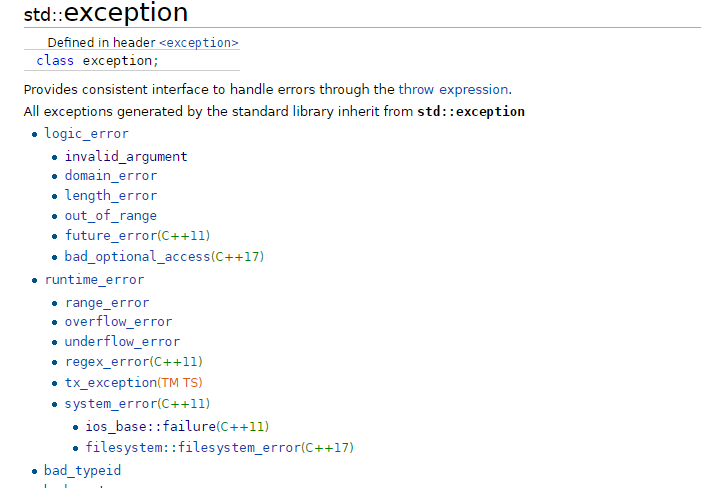
\includegraphics[scale=0.55]{fig/rc6stdexp}
\end{figure}
\end{frame}

\begin{frame}{Tips}
\begin{enumerate}
	\item Throw by value and catch by const reference.
	\item \texttt{throw} only on real exceptions
\end{enumerate}
\begin{block}{Throw by value}
	When an exception is raised, the programming is doing sort of recovery. The function that throws the exceptions most likely is going to terminate.
	Thus throwing reference (or address) to local objects won't make sense at the handling site.  
\end{block}
\begin{block}{Catch by const reference}
	The very reason that you need to catch exceptions by reference is simply because exceptions can contain virtual functions.
\end{block}
\end{frame}


%\begin{frame}[fragile]{Problems with exception}
%\structure{Quotation from Google C++ Style Guide:}
%\begin{quotation}
%	\alert{We do not use C++ exceptions}. ... Our advice against using exceptions is not predicated on philosophical or moral grounds, but practical ones. ... Things would probably be different if we had to do it all over again from scratch.
%\end{quotation}
%
%\structure{The Criticism}
%
%Again we quote from the same document:
%\begin{quotation}
%	When you add a throw statement to an existing function, you must examine all of its transitive callers. Either they must make at least the \alert{basic exception safety guarantee}, or they must never catch the exception and be happy with the program terminating as a result.
%\end{quotation}
%
%\tiny{\verb|https://google.github.io/styleguide/cppguide.html#Exceptions|}
%\end{frame}
%
%\begin{frame}[fragile]{Exceptions causing problem}
%Consider the following code:
%\begin{minted}{c++}
%
%\end{minted}
%\end{frame}
%
%
%\begin{frame}[fragile]{Exception Safety}
%There are in general 3 levels of exception safety:
%\begin{description}[No-throw Guarantee]
%	\item[No-throw Guarantee] The function will not throw an exception or \alert{allow one to propagate}. 
%	\item[Strong Guarantee] If a function terminates because of an exception, it will not leak memory and no data will not be modified, if it has never been called from the beginning.
%	\item[Basic Guarantee] If an exception is thrown, no resource (memory) is leaked ... though the data might have been modified.
%\end{description}
%
%Understand these guarantees as part of the specification for your function. Exceptions allows the function to interact with the outside world (by throwing exceptions) and it requires the outside world to change accordingly (catch exceptions).
%
%\tiny{From MSDN 0\verb|https://msdn.microsoft.com/en-us/library/hh279653.aspx|}
%\end{frame}


